\section{Methods}

For a user $U_i$ with posts $[P_{i,1}, P_{i,2}, ..., P_{i,n}]$ in the activity history, where $n$ is the number of total posts and $P_{i,j}$ is the $j$-th user-generated post of $U_i$, the goal of \textit{conventional depression detection} is to predict a binary label $y_i \in \{0, 1\}$ indicating whether the user $U_i$ suffers from depression, given the whole activity history. In contrast, in an \textit{early risk detection} (ERD) setting, the posts come one by one, so that only $[P_{i,1}, P_{i,2}, ..., P_{i,t}]$ is available to the model at the $t$-th time. The model can make an early prediction of $y_i$ at $t (t \leq n)$ once it is confident enough, such that the prediction can make a good tradeoff between accuracy and earliness (with $t$ as small as possible). Our solutions for both settings are as follows. 

\subsection{Risky Post Screening}
\label{sec:screening}

A reddit user typically has hundreds or thousands of posts in the whole activity history. However, since not all user posts are relevant to the detection of depression, retaining all posts may run the risk of introducing distractors that can hinder model performance and efficiency. Therefore, effective post selection strategy can be crucial to the success of ERD. 

Intuitively, posts that directly disclose the state of depression or express depression-related symptoms would indicate high depression risks. These intuitions can be reliably captured by psychometrically validated clinical scales. Therefore, we draw inspiration from these scales, and devise \textbf{depression templates} to screen risky posts out of the lengthy activity history. Only the posts with highest similarities to these templates will be selected as risky posts for further prediction.

Our depression templates are made up of 2 groups of descriptions. 
The first group consists of 3 explicit depression-related expressions: 
``I feel depressed'', ``I am diagnosed with depression'', 
``I am treating my depression'', matching the person's claim of 
general depressive mood, the diagnosis and the post-diagnosis treatment,
respectively. The second group is comprised of descriptions corresponding 
to dimensions defined in a clinical depression scale. 
Here we mainly adopt BDI-II, which is one of the most widely used depression 
measures\footnote{We also experimented with other scales and combinations of multiple scales, see Appendix for more details.} \cite{beck1996beck}. 
The scale includes the descriptions of four different intensities for each of the 21 symptoms. For example, ``1: I do not feel sad'', ``2: I feel sad much of the time'', ``3: I am sad all the time'' and ``4: I am so sad or unhappy that I can't stand it'' for the symptom of sadness. However, we find that current sentence representations have difficulty in capturing such nuanced differences. Therefore, we make slight manual modifications on them to construct a single representative template for each dimension, like ``I feel sad'' for Sadness. We provide examples in Table \ref{tab:template_example}.

\begin{table}[h]
    \centering
    \begin{tabular}{l|l}
        \hline
        Dimension & Template \\
        \hline
        Crying & I always cry. \\
        Tiredness  & I am too tired to do things. \\
        Self-Dislike & I am disappointed in myself. \\
        \hline
    \end{tabular}
    \caption{Example BDI-II dimensions and their corresponding templates.}
    \label{tab:template_example}
\end{table}

To measure the similarity between posts and depression templates, we resort to pretrained sentence-transformers \cite{reimers-2019-sentence-bert} to get the sentence representations, and calculate the cosine similarity between each post-template pair. For a post, its most similar template is referred to as its \textbf{diagnostic basis}, and their similarity is regarded as the \textbf{risk} of the post. The process of \textbf{risky post selection} is to select at most $K$ posts with the highest risks out of all posts of a user. Since the procedure consists of only sentence encoding from a pretrained model, and cosine similarity calculations, our method can be more efficient than previous works on post selection that requires costly RL training \cite{gui2019cooperative}. Moreover, the theoretical underpinning basis for post selection is also more effective than heuristic-based selection such as clustering \cite{zogan2021depressionnet}, as we will validate in the experiments (\S \ref{sec:conventional}).

\subsection{Hierarchical Attentional Network}
\label{sec:HAN}

Although depression detection can be formulated as text classification problem, it is different from conventional settings in that the input consists of multiple posts attached with temporal information. We may reformat the input by simply concatenating all posts. However, such representations will lost the time and structural clues at the post level, and also lead to a lengthy sequence. Further, conventional text classification models are lacking in explainability. 

To leverage the posting list structure as well as providing post-level explainability, we adopt the framework of Hierarchical Attentional Network (HAN) \cite{yang2016hierarchical} in our model design. The HAN consists of a post encoder and a user encoder. 

The post encoder takes the words $\{x_1, x_2, ..., x_L\}$ in a single post, and encode them into a post representation $p$. Thanks to the pre-step of risky post screening, we are able to take advantage of a large post encoder as opposed to shallow CNN or GRU based structures used in previous works \cite{yates2017depression,zogan2021explainable}. Hence we use a pretrained BERT model as the post encoder and the representation of the [CLS] token as the representation for the whole post. Therefore, the post encoder can be represented as: 

\begin{equation}
    p = BERT_{[CLS]}(x_1, x_2, ..., x_L)
\end{equation}

Given the representations of the $K$ risky posts $\{p_1, p_2, ..., p_K\}$, the user encoder models the relations between these posts as well as their chronological order to produce updated contextualized representations of each post $\{p'_1, p'_2, ..., p'_K\}$, and further aggregate these embeddings into one user representation $u$. Here we utilize a transformer structure to model the posts' relations with self-attention and encode the order with positional embeddings. The updated post representations are further passed to an attentional pooling layer, which learns the weight for each post embedding and perform a weighted sum of them accordingly, to get the final user representation. The attention mechanism can distinguish the contributions of each posts with learned weight so that important posts will have a higher influence on the final prediction. After all, the user encoder can be represented as:

\begin{equation}
    p'_1, p'_2, ..., p'_K = Transformer(p_1, p_2, ..., p_K)
\end{equation}
\begin{equation}
    \alpha_k = \frac{exp(W p'_k + b)}{\sum_{k'=1}^{K} exp(W p'_{k'} + b)}
\end{equation}
\begin{equation}
    u = \sum_{k=1}^K \alpha_k p'_k
\end{equation}
where $W$ and $b$ is learnable weight matrix and bias term of the linear transformation in the attentional pooling layer. Finally, a linear layer on top of the user representation makes the final binary classification of depression. The whole model is trained with the standard binary cross entropy loss.

With the HAN model above, most of the single post will not exceed BERT length limit. The attention weights can also provide explanations for which post is considered vital in the model's decision. % The computational complexity of self attention in transformer can also be reduced. Supposing the posting list has $K$ posts and their average length is $L$, a concatenated sequence would require $O(K^2 L^2)$ computations, while the complexity becomes $O(K^2 + K L^2)$ in the hierarchical model, which is significantly smaller if $K << L$, which holds in our typical settings ($K = 16, L = 128$).

\begin{figure*}[htbp]
    \centering
    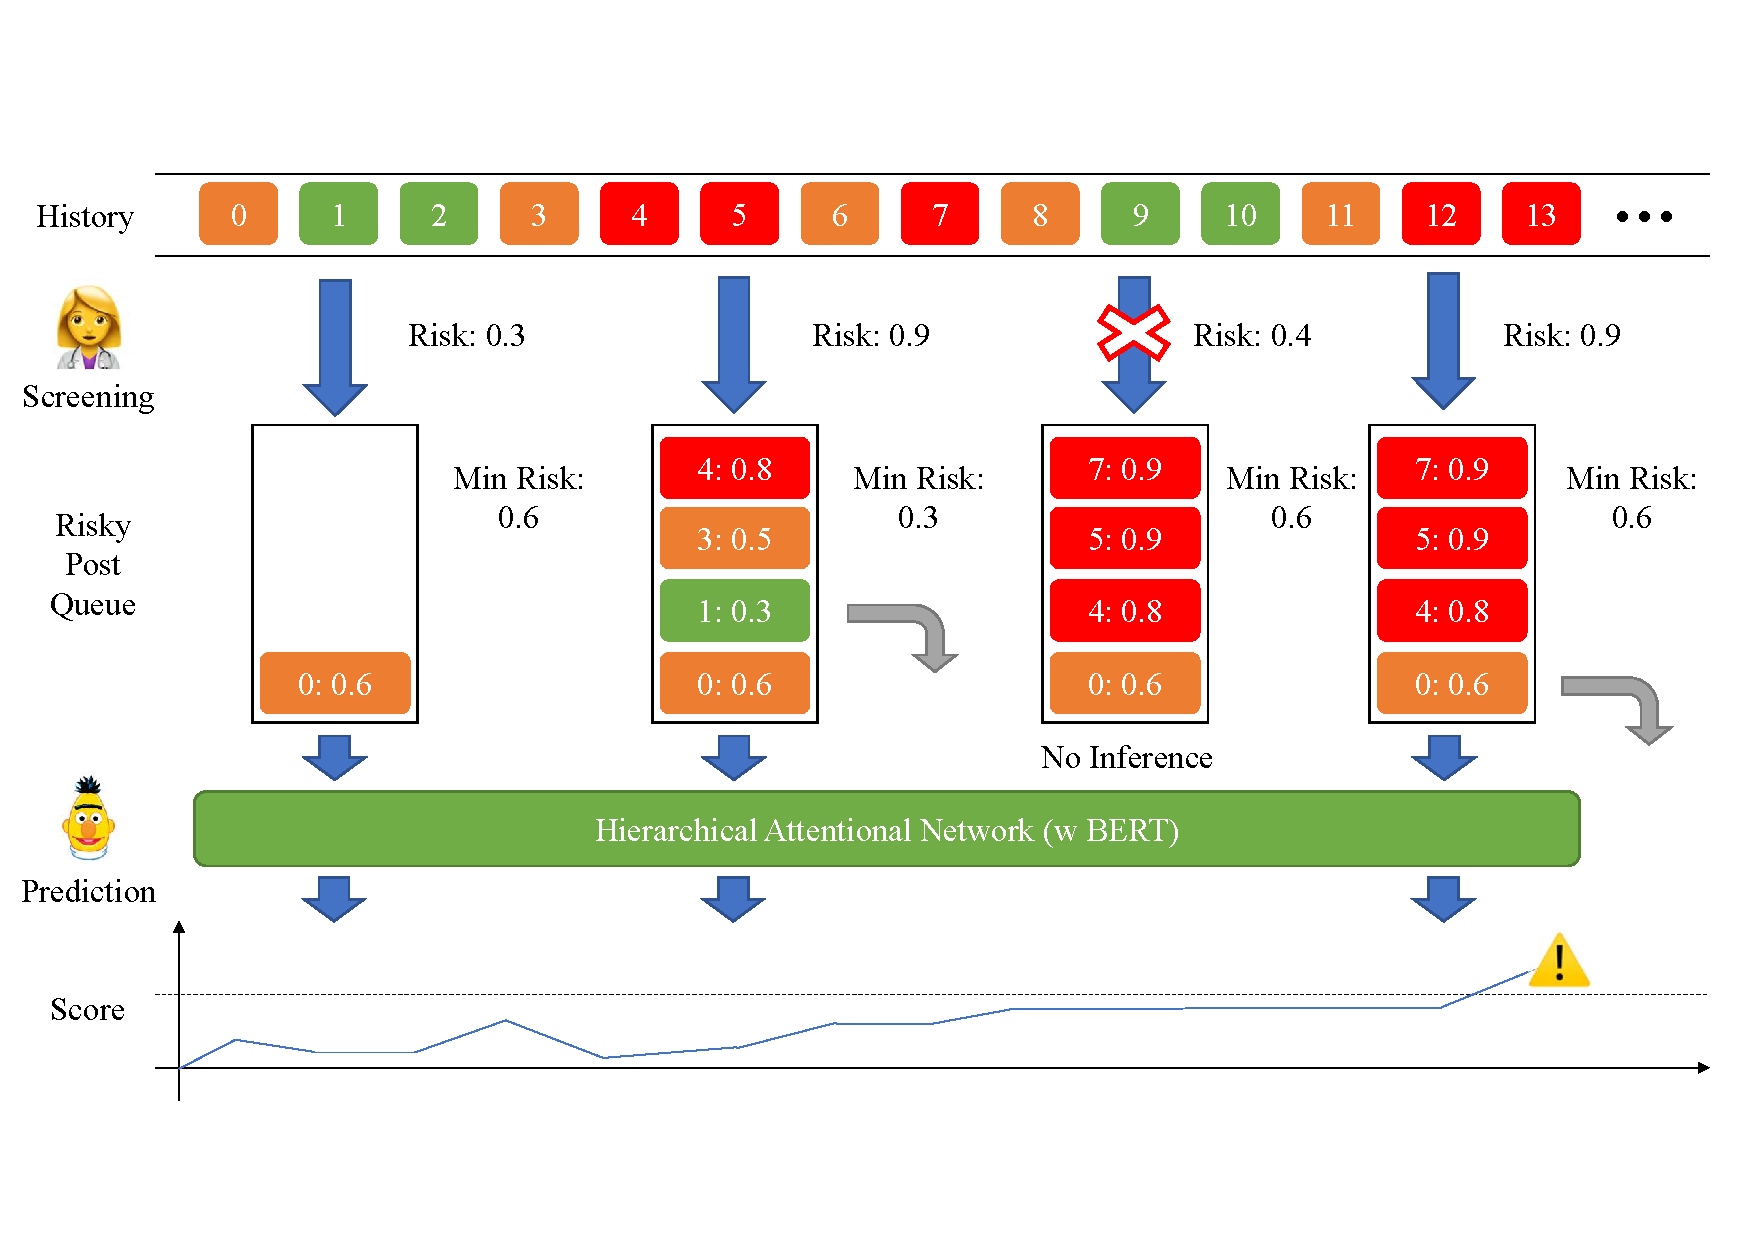
\includegraphics[width=1.5\columnwidth]{figures/evolving.pdf}
    \caption{Illustration of the evolving queue for early risk detection.}
    \label{fig:evolving}
\end{figure*}

\subsection{Evolving Queue for Early Detection}
\label{sec:evolving}

In an ERD scenario, we need to incrementally make predictions each time a user posts, instead of processing the whole posting history once.
This brings the computational challenges of frequent \textit{feature updates} and \textit{model inferences}. For example, a traditional feature-based model would have to recalculate the features like LDA topic distribution \cite{blei2003latent} from the whole activity history after each single update, and then make prediction accordingly. Such frequent recalculations can be even intractable for typical DNN solutions. Although post selection strategies can reduce the computational costs at the \textit{model inference} stage to some extent, the selection stage itself can become a performance bottleneck if it is not efficient enough. 

Moreover, the frequent updates may also be sensitive to one single depression-like post and easily produce false positive predictions, while the depressed patients tend to suffer from durative symptoms  \cite{kroenke2001phq} as opposed to control users who can also be depressive at some moments. Since the ERD setting does not allow modifying the prediction, once the model makes a confident diagnosis (since we may have already taken action to intervene in the dangerous situation), these false positives cannot be corrected later.

To tackle the above challenges, we further propose an online algorithm based on evolving queue of risky posts to adapt the above methods (\S \ref{sec:screening}, \S \ref{sec:HAN}) for effective and efficient early detection. First, the Risky Post Screening has already provided an efficient basis for the \textit{feature updates} step\footnote{We may view the selected posts as ``features'' in our model, since they are the actual inputs for the prediction model.}, as discussed above. However, the \textit{model inferences} remain computationally demanding. We observe that we don't have to make a prediction for each post, as some posts are not very helpful or even misleading for the detection of depression, and these posts are exactly what we would filter out with our screening approach as low risk posts. 
%% %myw This doesn't explain the reason why we need an evolving queue - it only states that we need to filter the unwanted posts, aka the previous risky post screening section. Make it clear that we only want the most risky posts and the number should be limited to reduce computational cost
Therefore, we can make prediction updates only if the new post is considered 
risky enough, so that the number of model inferences can be substantially reduced. The computational costs can be further contained by limiting the number of posts used in inference, so that only the most risky and recent posts will be included.

We implement the above intuition with an evolving queue updated according to 
post risk. The whole procedure is illustrated in Figure~\ref{fig:evolving}. 
We set the capacity of the queue to $K$ to control the computational costs 
as well as the number of posts used in training. 
For each incoming post $p$, the queue is updated according to the 
following rules: 
\begin{enumerate}
    \item If the queue is not full, we will add $p$ into the queue no matter how risky it is.
    \item If the queue has already been full, we will compare the risk of $p$ with the minimum risk of all posts in the queue. If $p$ is less risky, it will not be included in the queue. Otherwise, the least risky post in the queue will be removed for the insertion of $p$. The posts in queue will then be sorted in chronological order to align with the model's positional encoding.
\end{enumerate}

The HAN model will make inference only if the queue updates to avoid unnecessary computations. If the model's predicted probability exceeds a predefined threshold, it will report a early alert of depression and stop further calculations.
